% !TeX root = ../thuthesis-example.tex

\chapter{基于特征关系图的循环神经网络算法}
\section{引言}
从第2章的实验可以知道,现有的异常检测算法能够在公开数据集取得较为不错的表现,但是在真实数据集——清华大学校园网流量数据上效果均无法达到要求。这是因为相比于人工构造的公开数据集,清华大学校园网数据具有规模大、应用类型种类繁多、异常流量占比多、难以学到基线等特点。而RNN、LSTM、GRU等拟合能力强大的深度学习模型在校园网数据集中有着准确率低、误报率高的问题。因此本章将先从特征分析着手,分析RNN模型效果不佳的原因,然后引入特征之间的关系矩阵,将其加入到神经网络的训练中,从而获得更好的检测效果。

\section{特征分析}
模型可解释的分析方法通常有两类:
\begin{enumerate}
  \item 通过数学推导来解释每个特征如何发挥作用,例如线性回归中的系数,SVM中的支撑平面等,这类方法旨在分析因果关系。
  \item 针对神经网络等“黑盒”模型,通过分析特征如何影响最终预测结果,来部分解释模型的原因,这类方法旨在分析关联关系。
\end{enumerate}
本文中采用第二类方法,使用Shapley值这一工具来尝试解释RNN类模型在CAMPUS数据集中效果不佳的原因。
% \section{CAMPUS数据集和开源数据集的不同之处}
% 同样的算法和参数,在不同数据集上表现迥异,并且我们在多个数据集上都尝试了不同的参数。说明数据分布、类别存在差异,。并且变量的维度一致。

% 通过对比两者的不同,我们发现是因为缺乏特征关系。为此我们将分析特征关系。

% 下表为UNSW-NB15的攻击类型、每类攻击的占比。三个饼状图。
% 对攻击类型做个分类,发现不同之处。

% 寻找攻击类型和特征之间的关系,也就是通过实验发现哪些特征起到了作用。

% 得出结果:相比于其他两个数据集,CAMPUS数据集具有以下特点:

% 1.攻击类型更多更复杂。CICIDS数据集仅有7种攻击类型,UNSW-NB有9种。

% 2.在CAMPUS中特征和攻击类型的关联性更弱,需要进一步挖掘。(如何刻画特征和label之间的关联性)分别画图表示关联性强弱。


Shapley值起源于1953年的博弈论\cite{lundberg2018consistent},是为了解决这样一个问题:一群拥有不同技能的参与者为了集体奖励而相互合作。那么,如何在小组中公平分配奖励?在机器学习领域,参与者就是输入的特征,而集体奖励则是模型输出的结果。Shapley值可用于计算每个特征对于模型输出的贡献。其公式如下: 
\begin{equation}
  \phi_i(v) = \sum_{S\subseteq N \setminus \{i\}} \frac{|S|! (|N| - |S| - 1)!}{|N|!}(v(S \cup \{i\}) - v(S))
\end{equation}

其中,$N$是所有特征构成的集合,$S$是$N$的子集,$v(\cdot)$可以认为是模型,$\phi_i(v)$ 即为第i个特征的“重要性”。

本文利用python中的shap库\footnote{https://github.com/slundberg/shap}分别计算了RNN模型在三个数据集中的Shapley值,并从SHAP特征重要度、SHAP摘要图两方面进行了可视化分析。

SHAP特征重要度的原理是Shapley绝对值越大,其对应的特征越重要。由于公式3-1中计算得到的是单个实例的Shapley值,因此我们需要对每个特征的全部实例取平均值:
\begin{equation}
  I_j = \sum_{i=1}^n |\phi_j^{(i)}|
\end{equation}
% 图\ref{DT模型的特征重要度top20}和图\ref{RF模型的特征重要度top20}分别是DT和RF模型在UNSW-NB15数据集中的特征重要度排序,\ref{RNN模型的特征重要度top20}是RNN模型在CAMPUS数据集中的特征重要度排序。从中可以看出,两种树模型的前20个重要特征的重合度很高,都利用了sttl(源报文的ttl字段)、sbytes(会话中从源发出的总字节数)、synack(第一次发送报文到收到确认报文的时间)等特征,这些“强特征”对于模型判断某条流是否为异常提供了重要信息。而RNN模型在CAMPUS数据集上仅利用了极少数的特征。
图3.1和图3.2分别是DT和RF模型在UNSW-NB15数据集中的特征重要度排序,图3.3是RNN模型在CAMPUS数据集中的特征重要度排序。从中可以看出,两种树模型的前20个重要特征的重合度很高,都利用了sttl(源报文的ttl字段)、sbytes(会话中从源发出的总字节数)、synack(第一次发送报文到收到确认报文的时间)等特征,这些“强特征”对于模型判断某条流是否为异常提供了重要信息。而RNN模型在CAMPUS数据集上仅利用了极少数的特征。


% 接下来我们对每个特征重要度降序排序并且进行绘制,结果如图所示。从中可以看出,排名前列的特征更多是与报文大小相关的特征和报文发送时间相关的特征。通过协议分析得到的特征的重要性相对更弱。

% \begin{figure}
%   \centering
%   \includegraphics[scale=0.1]{mean-sharp-value.bmp}
%   \caption{shap-importance}
%   \label{fig:shap-importance}
% \end{figure}

\begin{figure}[htbp]
  \centering
  \begin{minipage}[t]{0.48\textwidth}
  \centering
  % \label{DT模型的特征重要度top20}
  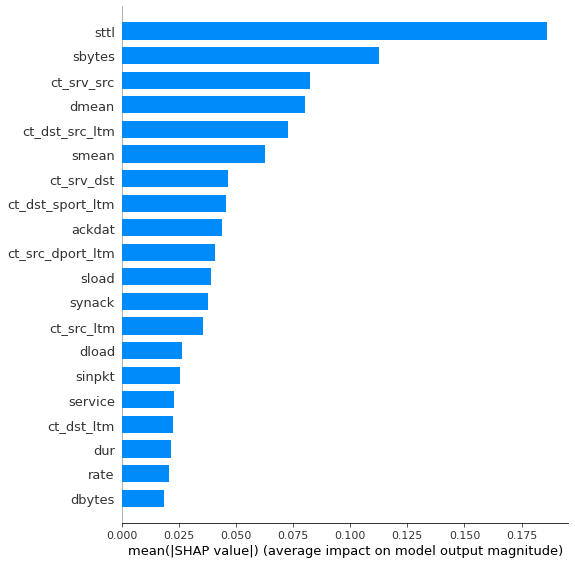
\includegraphics[scale=0.4]{DT-import-1000.png}
  \caption{DT模型的特征重要度top20}
  
  \end{minipage}
  \begin{minipage}[t]{0.48\textwidth}
  \centering
  % \label{RF模型的特征重要度top20}
  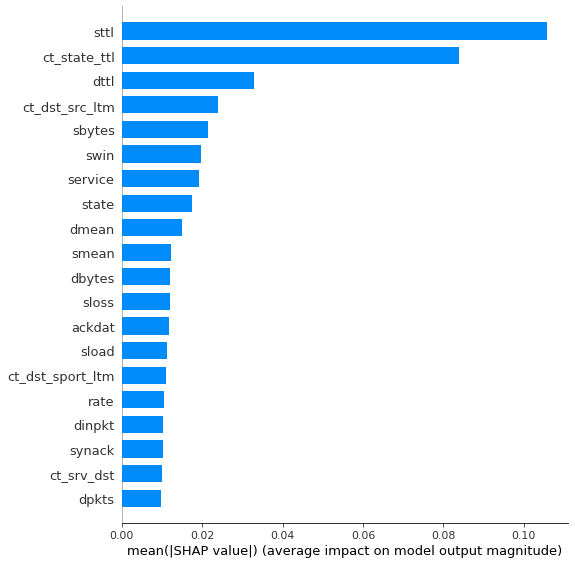
\includegraphics[scale=0.4]{RF-import-1000.png}
  \caption{RF模型的特征重要度top20}
 
  \end{minipage}

  \begin{minipage}[t]{0.48\textwidth}
    \centering
    % \label{RNN模型的特征重要度top20}
    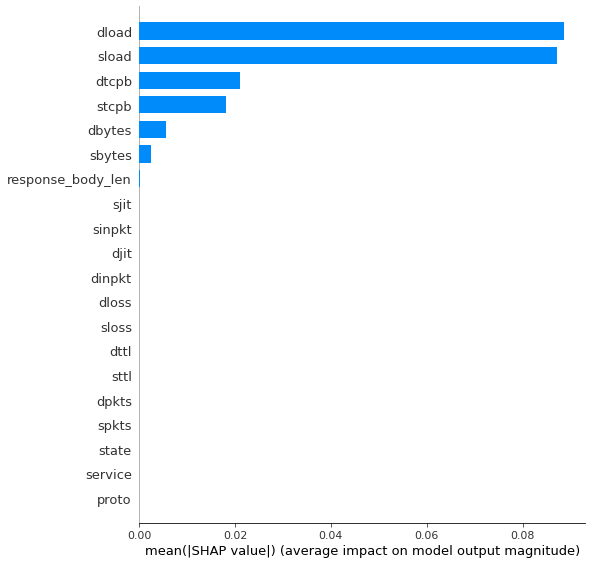
\includegraphics[scale=0.4]{NN-import-1000.png}
    \caption{RNN模型的特征重要度top20}
    
    \end{minipage}
  \end{figure}


% 由图中可以看出,在CAMPUS数据集中,特征间重要程度呈现均衡化。

图3.4-3.6是SHAP摘要图。SHAP摘要图将特征影响和特征重要度结合起来。摘要图上的每个点都是一个特征和一个实例的Shapley值,y轴上的位置由特征决定,x轴上的位置由Shapley值决定,颜色代表特征值从小到大,重叠点在y轴方向上抖动,因此我们可以了解每个特征的Shapley值的分布。例如sttl这一特征,红色说明特征值很高,在图中sttl很高时,其SHAP值为0,说明对预测结果影响很小,这点也符合我们的认知。从图中对比可以看出,RNN模型的大部分特征的SHAP值都为0。

% \begin{figure}
%   \centering
%   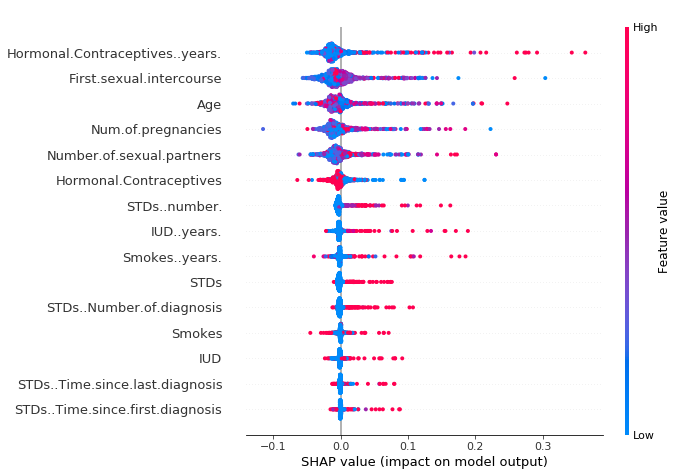
\includegraphics[scale=0.5]{shap-importance-extended.png}
%   \caption{shap-importance-extended}
%   \label{fig:shap-importance-extended}
% \end{figure}

\begin{figure}[htbp]
  \centering
  \begin{minipage}[t]{0.48\textwidth}
  \centering
  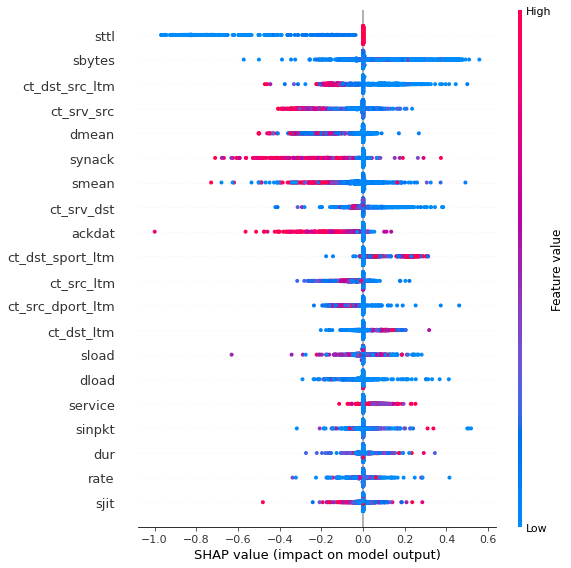
\includegraphics[scale=0.4]{DT-shap-value-1000.png}
  \caption{DT模型在UNSW中的摘要图}
  \end{minipage}
  \begin{minipage}[t]{0.48\textwidth}
  \centering
  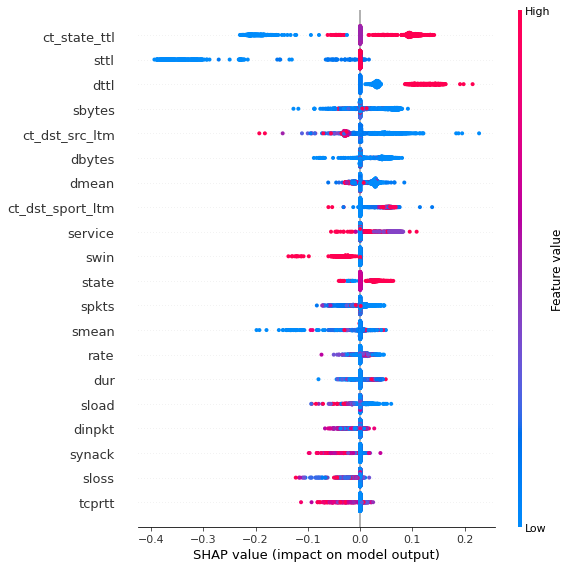
\includegraphics[scale=0.4]{RF-sha-value-1000.png}
  \caption{RF模型在UNSW中的摘要图}
  \end{minipage}

  \begin{minipage}[t]{0.48\textwidth}
    \centering
    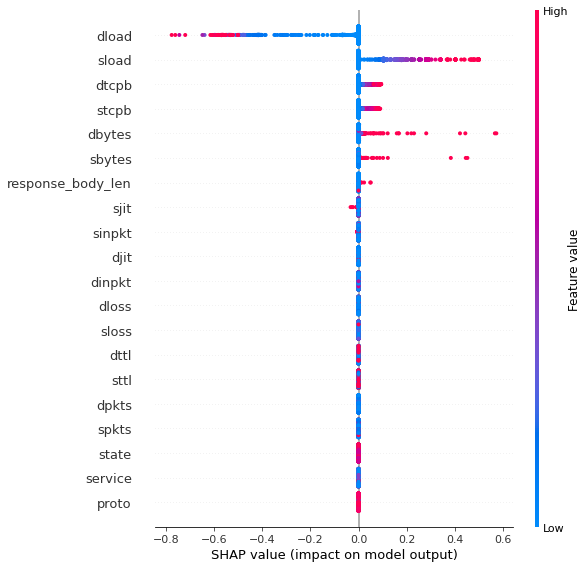
\includegraphics[scale=0.4]{NN-shap-value-1000.png}
    \caption{RNN模型在CAMPUS中的摘要图}
    \end{minipage}
  \end{figure}

% SHAP依赖图刻画了全部实例的某个特征值和Shapley值之间的关联。

通过本节的分析,我们得出以下结论:
\begin{enumerate}
  \item SHAP特征重要度和摘要图可以一定程度的解释模型。
  \item 对比不同的数据集,树模型中top20重要性的特征相似,说明这些“强特征”更能影响检测结果。
  \item 在CAMPUS数据集中,相比于其他模型,RNN仅利用到了少部分特征信息。
\end{enumerate}
% 特征分析结论:
% SHAP特征重要性和摘要图可以一定程度的解释模型;
% 对比不同的数据集,树模型中top20重要性的特征相似,说明这些“强特征”更能影响检测结果;
% 在CAMPUS数据集中,相比于其他模型,RNN仅利用到了少部分特征信息。

% 1.DNN算法在CAMPUS数据集上失效的原因之一是训练过程中特征重要度相近,没有哪个。2.其他算法的top10特征都是相似的,DNN没有这样。 这也是RNN没有从数据中学习出特征关系的印证。

% \begin{figure}[htbp]
  % \centering
  % \begin{minipage}[t]{0.48\textwidth}
  % \centering
  % 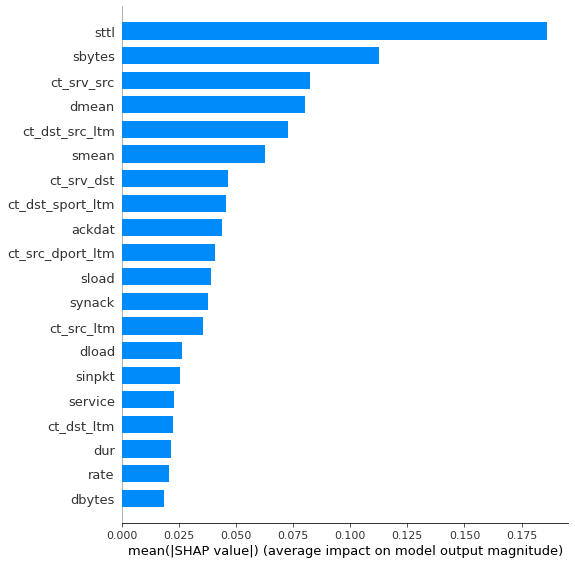
\includegraphics[scale=0.4]{DT-import-1000.png}
  % \caption{DT模型的特征重要度top20}
  % \end{minipage}
  % \begin{minipage}[t]{0.48\textwidth}
  % \centering
  % 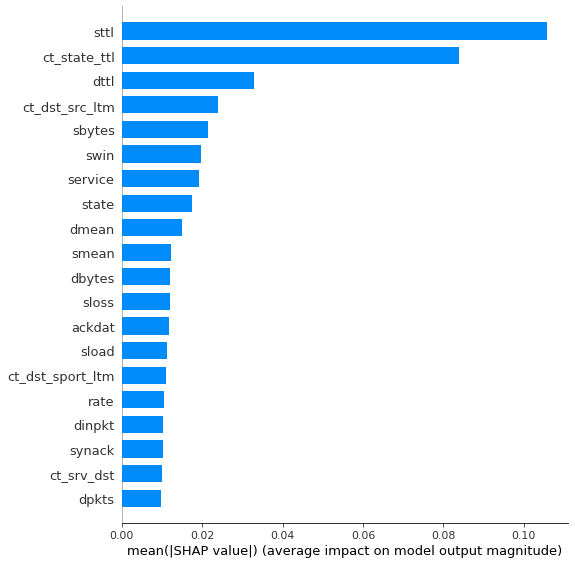
\includegraphics[scale=0.4]{RF-import-1000.png}
  % \caption{RF模型的特征重要度top20}
  % \end{minipage}

  % \begin{minipage}[t]{0.48\textwidth}
  %   \centering
  %   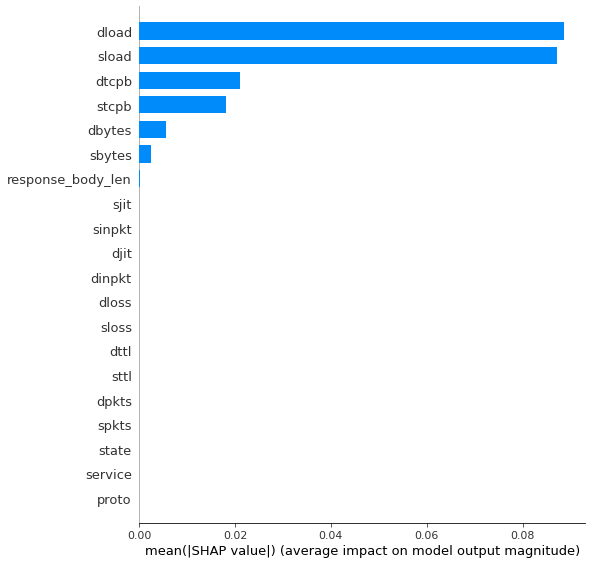
\includegraphics[scale=0.4]{NN-import-1000.png}
  %   \caption{NN模型的特征重要度top20}
  %   \end{minipage}
  % \end{figure}

% 从两方面分析:分别用同样的算法在不同数据集上对比。
\section{特征关系}
流量特征可以视为反映当前网络流量的一组观察值,从多个角度描述当前的流量场景。好的特征能够真实地反映出流本身的状态信息。例如对于一条单个TCP流,这条流可能是一个正常的端到端的连接,也可能是分布式拒绝服务攻击的一部分,在被攻击者的视角内,它的入流量的带宽急剧增加,且远大于出流量的带宽。
% 图\ref{fig:特征关系}表示某一时刻下部分特征之间的关系,从中我们看出,发送方/接收方数据包长度大小与流的传输速率具有很强的关联性。

% \begin{figure}
%   \centering
%   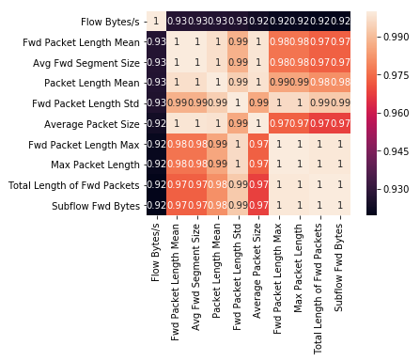
\includegraphics[scale=1]{特征关系.png}
%   \caption{特征关系}
%   \label{fig:特征关系}
% \end{figure}

我们分析了暴力猜解攻击的部分特征信息,从表\ref{暴力猜解case分析}中可以看出,相比于正常流量,当发生暴力猜解攻击时,其从源报文发出的总字节数(sbytes)和源报文的间隔时间的平均值(sinpkt)都非常小。在这种场景下,sbytes和sinpkt的关联性更强,而在正常流量场景下两者的关联性更弱。

\begin{table*}[h]
  \small
  \caption{暴力猜解case分析}
  \label{暴力猜解case分析}
  \centering
  \begin{tabular}{cccccccc}
  \toprule
  dur & proto & sbytes & dbytes & sinpkt & dinpkt & ... & attack type \\
  % 会话持续时间 & 协议 & \tabincell{c}{从源发出的\\总字节数} & \tabincell{c}{从目的发出的\\总字节数} & \tabincell{c}{源报文的间隔\\时间的平均值} & \tabincell{c}{目的报文的间隔\\时间的平均值} & 。。。 & 攻击类型 \\
  \midrule
  0.216048 &	113	&990	&2038	&24.005333	&28.037572 & ... & Normal\\
  0.824394	&113	&1054	&1344	&43.335262	&42.801578 & ... & Normal\\
  0.000007	&119	&114	&0	&0.007	&0 & ... & Generic\\
  0.000007	&119	&114	&0	&0.007	&0 & ... & Generic\\
  0.000005	&119	&120	&0	&0.005	&0 & ... & Generic\\
  
   \bottomrule
  
  \end{tabular}
  \end{table*}
  

由上节的分析可知,在CAMPUS数据集中,RNN仅利用了极少数的特征信息,为了捕获更多特征信息,因此需要挖掘特征之间的潜在关联。从本质上来说,各种机器学习、深度学习模型就是挖掘特征信息的过程。然而针对CAMPUS数据集,RNN模型无法有效提取信息,通常的做法有两种:
\begin{enumerate}
  \item 从特征工程着手,进行特征组合或者特征交叉(Feature Crosses)。如果直接进行特征组合,则复杂度过高,需要$O(N^2)$的计算复杂度,并且导致维度爆炸。因此常用的方法有因子分解机(Factorization Machines),对于每个原始特征,FM都会学习一个隐向量。FM通过穷举所有的特征对,并进行逐一检测特征对的权值来自动识别出有效的特征组合。
  \item 从模型结构着手,在神经网络中增加额外辅助信息。例如机器翻译领域往往会加入文章的关键词、摘要等信息。这部分信息会影响到模型对于神经元参数的计算,从而影响特征权重。
\end{enumerate}

这两种做法各有优劣,方法1可以在线性时间内完成,但是只能对特征进行两两组合,并且组合信息难以进行解释;方法2能够捕捉到更多的关联信息,因此会增加神经网络的复杂性,带来额外的计算开销。由于本文使用的模型为预训练模型,无需在线实时训练,相比于几小时的模型训练时间,这部分计算延迟可以忽略,我们采用方法2挖掘特征潜在关系。

为了在神经网络中引入特征关系矩阵,本文利用皮尔逊相关系数来计算流量特征之间的关系。皮尔逊相关的别名是积差相关(或者称之为积矩相关),命名来源是20 世纪英国的描述统计学派先驱皮尔逊。对于两个变量X、Y,它们之间的皮尔逊相关系数为:
% 对于计算变量之间的线性相关性,他想到了一种方法,即假设当前存在两个变量X、Y,通过下列公式计算X、Y之间的皮尔逊相关系数:

% 皮尔逊相关也称为积差相关(或积矩相关)是英国统计学家皮尔逊于20世纪提出的一种计算线性相关的方法。

% 假设有两个变量X、Y,那么两变量间的皮尔逊相关系数可通过以下公式计算:
\begin{equation}
  \rho_{X,Y} = \frac{cov(X,Y)}{\rho_X\rho_Y}=\frac{E(XY)-E(X)E(Y)}{\sqrt{E(X^2)-E^2(X)}\sqrt{E(Y^2)-E^2(Y)}}
\end{equation}
其取值范围为[-1,1],$\rho_{X,Y}=1$时,说明X和Y完全正相关,$\rho_{X,Y}=-1$时,说明X和Y完全负相关,$\rho_{X,Y}$接近0时,说明X和Y无线性相关性。





\section{基于关系图结构的RNN}
由前两节分析可知,LSTM和GRU作为两种循环神经网络,都可以很好地提取时序相关性。但是在复杂的清华大学校园网流量环境下,仍然有很多改进空间。根据第2章的实验结果,LSTM和GRU在CAMPUS数据集下准确率仅为56.59\%和59.28\%。经过特征分析,我们发现不同时刻下特征之间的相关性会发生变化。因此本文中我们利用循环神经网络(RNN)对时间依赖性进行建模的同时对特征关系也进行建模。值得指出的是,本文中使用的RNN子类是“门控循环单元”(GRU),相比于普通RNN,它可以很好地捕捉到时序数据中相隔较远的依赖关系\cite{li2017diffusion}。在GRU的矩阵乘法中,我们加入了前文提到的特征关系图(Feature Graph)。

定义无向权重图$G=(V,E,W)$,其中$V$表示特征节点的集合,$|V|=N$; $E$表示特征间的关联关系,即图中的边;$W \in R[N*N]$为特征节点的相似度的加权邻接矩阵,我们称$W$为特征关系矩阵。将时刻t观察到的流量特征向量表示为$X^t$。那么流量预测目的就是:给定$G$下,学得一个函数将$T$个历史图信号映射到未来$T$时刻的图信号:
\begin{equation}
    h[X^{t-T+1}, X^{t-T+2},...,X^{t}; G] \Rightarrow [X^{t+1}, X^{t+2}, ..., X^{t+T}]
\end{equation}

\begin{equation}
    r^{(t)} = \sigma(\Theta_r\star G[X^{(t)},H^{t-1}] + b_r)
\end{equation}

\begin{equation}
    u^{(t)} = \sigma(\Theta_u\star G[X^{(t)},H^{t-1}] + b_u)
\end{equation}

\begin{equation}
    C^{(t)} = tanh(\Theta_C\star_G[X^{(t)},(r^{(t)}\odot H^{(t-1)})] + b_c)
\end{equation}

\begin{equation}
    H^{(t)} = u^{(t)}\odot H^{(t-1)} + (1 - u^{(t)}) \odot C^{(t)}
\end{equation}

其中$X^{(t)}$, $H^{(t)}$表示在时间 $t$ 的输入和输出,$r^{(t)}$ $u^{(t)}$分别是在时间 $t$的复位门和更新门,$\star G$  表示扩散卷积。与GRU相似,该模型可用于构建递归神经网络层,并使用反向传播进行训练。
FG-RNN算法的原理如图\ref{fig:FG-RNN原理图}所示。
\begin{figure}[H]
  \centering
  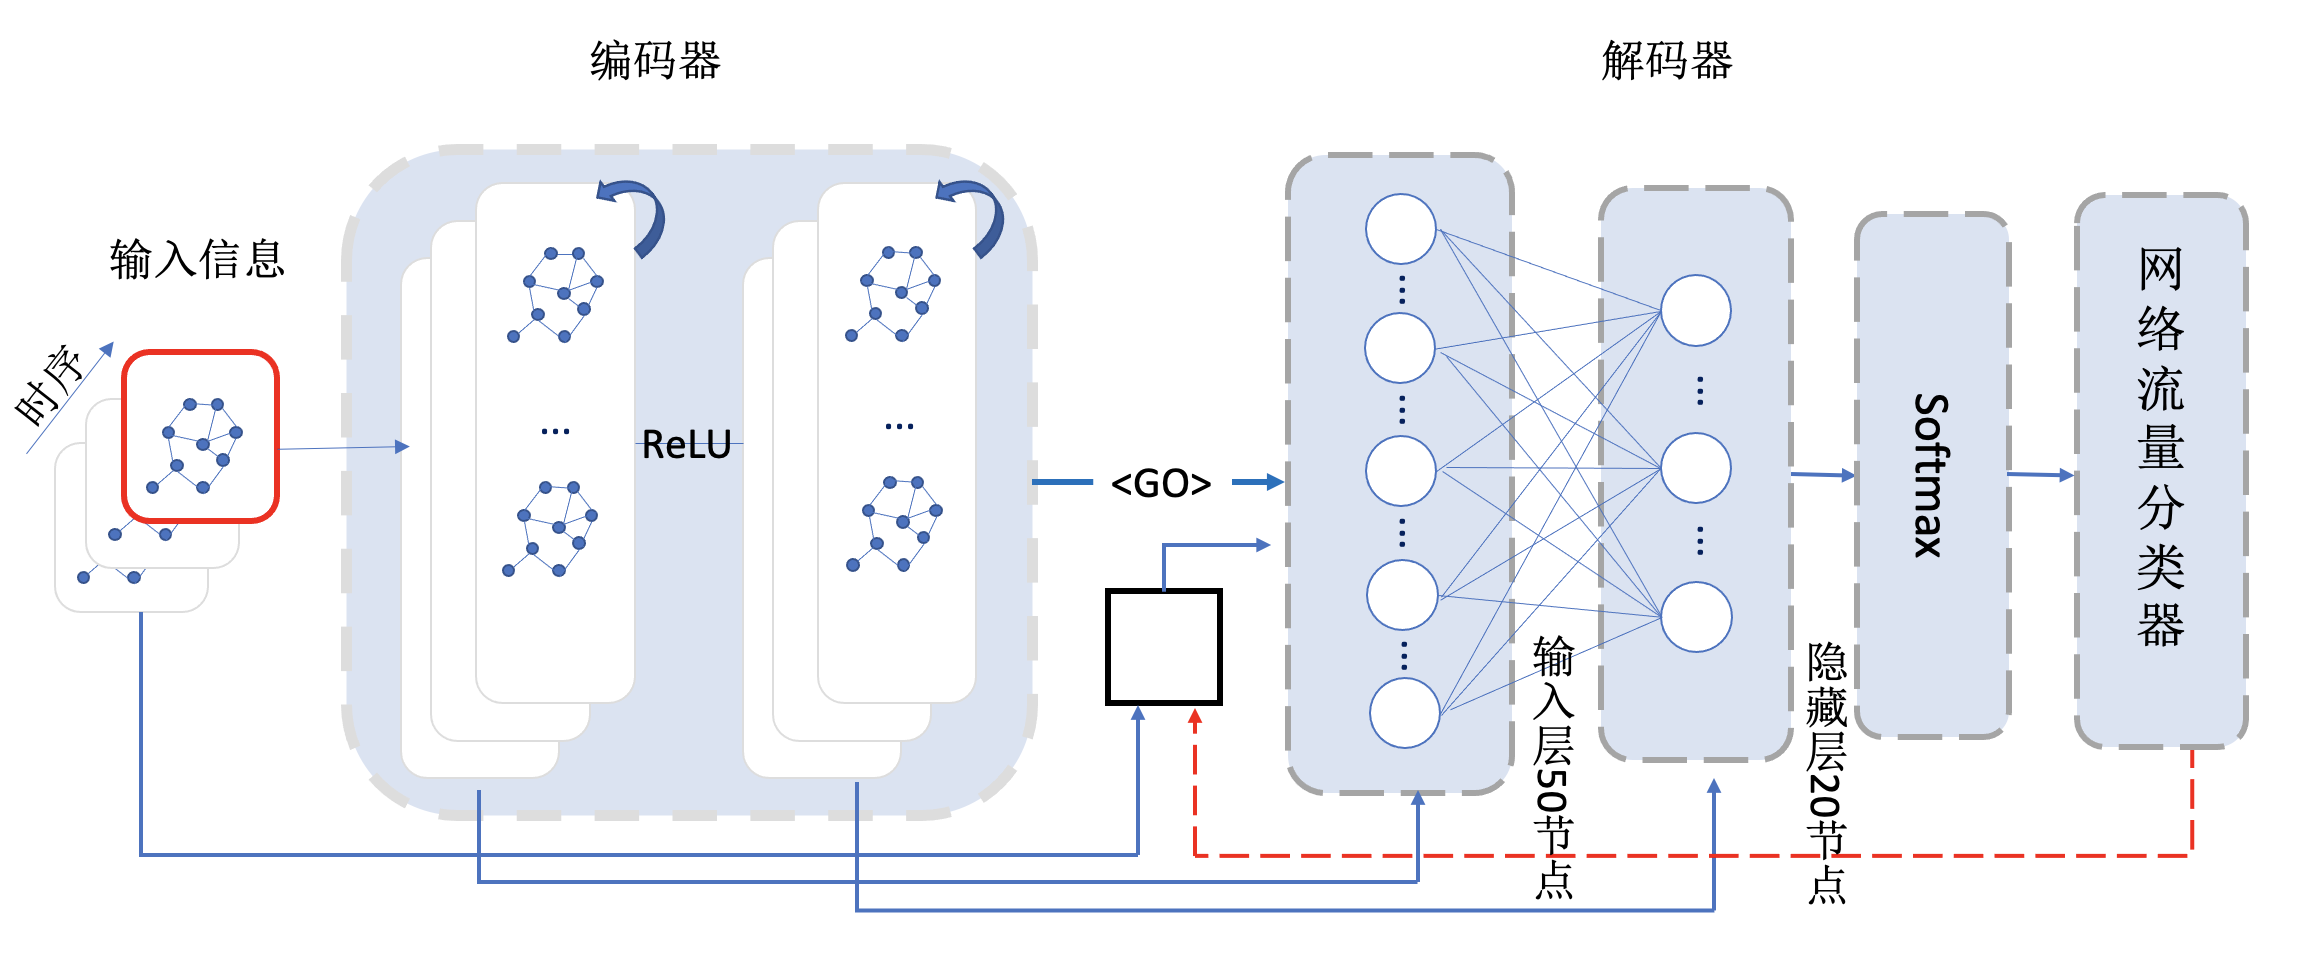
\includegraphics[width=1\linewidth]{FG-RNN原理图.png}
  \caption{FG-RNN原理图}
  \label{fig:FG-RNN原理图}
\end{figure}

在接下来的多步预测中,我们采用了seq2seq结果\cite{sutskever2014sequence}。编码器和解码器都是使用具有GRU的递归神经网络。 在训练过程中,我们将历史时间序列输入到编码器,并使用其最终状态来初始化解码器,解码器根据先前的观测值生成预测值。在检测时,真实值与模型生成的预测值进行对比,差异过大则为异常。 训练集和测试集分布之间的差异会导致性能下降。 为了解决这个问题,我们将预采样\cite{bengio2015scheduled}集合到模型中,其中,我们向模型提供概率为$\epsilon_i$的真实观测值或者 第i次迭代时模型以概率为$1-\epsilon_i$进行预测。 在训练过程中,$\epsilon_i$逐渐减少到0,以不断逼近真实观测值的数据分布。

FG-RNN算法的伪代码如算法\ref{FG-RNN伪代码}所示。本算法的核心代码已上传到github平台\footnote{https://github.com/GTnull/FG-RNN}。
\begin{algorithm}[!h]
  \caption{\emph{FG-RNN伪代码}}
  \label{FG-RNN伪代码}
  \begin{algorithmic}[1]
    \Require
      一组按时间排序的向量组$\vec{x_1}$,$\vec{x_2}$,...,$\vec{x_T}$,特征间关系图$G$以及它的邻接矩阵$W$

    \Ensure
      按时间排序的向量组$\vec{h_1}$,$\vec{h_2}$,...,$\vec{h_T}$
    \State 通过Xavier方法初始化$q_{net1}$, $q_{net2}$ and $p_{net}$的所有参数
    \While {$\mathcal{L}$没有收敛}
        \State 利用公式 计算每一个节点$v$的$q_{net1}$, $q_{net2}$ and $p_{net}$
        \For{i $\leftarrow$ $1$ to $T$}
        \State 更新特征关系矩阵$W(e)$的系数
        \State 更新GRU中的参数$W(X)$
        \State 计算$tanh(W(e) + W(X) + b)$        
        \EndFor
        \State 用公式计算目标函数$\mathcal{L}(\theta, \phi)$ 
        \State 用梯度下降法更新$q_{net1}$,$q_{net2}$和$p_{net}$的所有参数
    \EndWhile
    %\State \Return $P_{net}$
  \end{algorithmic}
\end{algorithm}

通常,计算卷积会很费时。 但是,如果$G$很稀疏,则可以使用总时间复杂度 $O(K \mid \varepsilon \mid) \ll O(N^ 2)$ 递归稀疏矩阵乘法来有效地进行计算,本文中计算特征关系图和GRU都可以使用该矩阵乘法。


\section{FG-RNN收敛性证明}
在普通RNN的训练中,使用不正确的学习率、初始化权重发生错误、在输出层使用错误的激活函数等,均可能会导致模型最终无法收敛。而FG-RNN在RNN中加入了特征图信息,是否在一定条件下能够收敛呢?本节参考了Loukas等人对GNN收敛性的证明\cite{loukas2019graph},证明了FG-RNN在网络深度和宽度达到一定条件下时始终可以收敛。此证明过程也为后续模型训练前的超参数设置提供了指导。

% 在图神经网络中,目标节点的特征是根据它邻近节点的特征计算而来。

我们认为收敛的网络就是计算可达的网络。计算可达是指可以通过计算的方式,把输入数据输出成人们指定的结果。以图像识别为例,输入数据是一张图,输出数据是判断这幅图中是否有人/猫/狗等物,计算的载体则是深度学习模型。如果该网络模型经过海量数据学习,可以完全正确地完成图片分类任务,那么这个网络就是计算可达的。假设存在一个理想化的映射$f(\cdot)$,对任何输入的图像,它都能给出一个正确的分类结果。将我们的模型学习出来的复杂神经网络抽象为映射$g(\cdot)$。计算可达就是指$g(\cdot)$无限接近于$f(\cdot)$,即$||f(\cdot) - g(\cdot)|| \rightarrow 0$。后续我们称这个理想化映射为模型$LOCAL$。

首先,我们给出待证明的命题和已知条件:
\begin{itemize}
  \item 待证明的命题:FG-RNN在条件$X$下是计算可达的,条件$X$是未知的。
  \item 已知条件:计算模型$LOCAL$在条件$Y$下是计算可达的,条件$Y$是已知的。
\end{itemize}


其中$LOCAL$ 是一个计算复杂度非常高的理想化网络模型,其每个节点的信息在每次迭代中都会传递给其余全部近邻点,可以把它想象成一个细胞间传递信息的生物模型。它的计算过程的伪代码如算法\ref{LOCAL伪代码}所示。
\begin{algorithm}[!h]
  \caption{\emph{LOCAL伪代码}}
  \label{LOCAL伪代码}
  \begin{algorithmic}[1]
    % \Require
    %   一组按时间排序的向量组$\vec{x_1}$,$\vec{x_2}$,...,$\vec{x_T}$, 特征间关系图$G$以及它的邻接矩阵$W$

    % \Ensure
    %   按时间排序的向量组$\vec{h_1}$,$\vec{h_2}$,...,$\vec{h_T}$
    \State 初始化参数,$s_{i\leftarrow i}^{(0)}=(a_i, v_i)$,$s_{i\leftarrow j}^{(0)}=(a_j, v_j)$
    \For {$round l = 1, 2, ..., d$}
        \State 从上一轮的所有近邻点接收状态,receive过程,$s_{i\leftarrow j}^{(l-1)}$ from $v_j \in N_i^*$
        \State 计算当前节点状态 $s_i^{(l)} = {ALG}_l^1 \big(\big\{\big(s_j^{(l-1)}, v_i, v_j,  a_{i\leftarrow j}\big): v_j \in N_i^* \big\}\big)$
        \State 将当前状态节点更新到其余节点,send过程, $s_{j\leftarrow i}^{(l)} = {ALG}_l^2 \big(s_i^{(l)}, v_i \big)$
    \EndFor
    %\State \Return $P_{net}$
  \end{algorithmic}
\end{algorithm}

在$LOCAL$算法中,$s_i$和$s_j$分别表示节点$v_i$的状态,运算符$ALG$表示一个图灵完备的算法,符号$N_i^*$表示目标节点的近邻点的集合。可以将每一个节点都假想成一个小细胞,这些细胞彼此紧紧地挨在一起。Receive过程就是目标细胞接受周围邻近细胞发出的化学物质的过程,Send过程就是目标细胞向周围邻近细胞发出的化学物质的过程。实际网络中这样的计算开销会以指数计,因此$LOCAL$是一个理想化的计算模型。
 
接下来我们只需要试图构造一个条件$Z$,在条件$Z$下,FG-RNN和$LOCAL$是等价的。这样,FG-RNN计算可达的条件就是$Y+Z$。
因此,我们按照以下步骤来证明:
\begin{enumerate}
  \item 证明在条件$Z$下,FG-RNN与$LOCAL$模型等价。
  \item 根据$LOCAL$的性质,证明在满足条件$Y$的情况下,$LOCAL$计算可达。
  \item FG-RNN计算可达的条件就是$Y+Z$。
\end{enumerate}

首先证明在条件$Z$下,FG-RNN与$LOCAL$等价,条件$Z$是指FG-RNN中的feature graph计算函数FG和权重更新函数UP都是图灵完备函数。

从FG-RNN 计算模型推导:
\begin{equation}
  \begin{aligned} 
  x_i^{(l)} &= UP_l \big(\sum_{v_j \in N_i^* m_{i\leftarrow j}^{(l)}} \big) \\
    &= UP_l \big(\sum_{v_j \in N_i^*} FG_l \big( x_i^{l-1}, x_j^{l-1}, v_i, v_j, a_{i\leftarrow j}\big) \big) \\
    &= AGG_l \big( \big\{ \big( x_i^{l-1}, x_j^{l-1}, v_i, v_j, a_{i\leftarrow j}\big) : v_j \in N_i^* \big\} \big)
  \end{aligned}  
\end{equation}
其中AGG是聚合函数,可以理解为是FG和UP的融合形式。

从$LOCAL$计算模型推导:
\begin{equation}
  \begin{aligned}
    s_l^{(l)} &= ALG_l^1 \big( \big\{ \big( s_{i\leftarrow j}^{(l - 1)}, a_{i\leftarrow j}\big) : v_j \in N_i^* \big\}, v_i\big) \\
    &= ALG_l^1 \big( \big\{ \big( \big( ALG_l^2 \big( s_j^{(l-1)}, v_j\big) \big), a_{i\leftarrow j}\big) : v_j \in N_i^* \big\}, v_i\big) \\
    &= ALG_l \big(\big\{\big(s_j^{(l-1)}, v_i, v_j,  a_{i\leftarrow j}\big): v_j \in N_i^* \big\}\big)
  \end{aligned}
\end{equation}

可以发现,两个计算模型可以推导出一种类似的形式。$ALG$的定义为一种图灵完备函数,而已知的FG和UP属于图灵完备函数,那么它们的复合函数AGG也是图灵完备的。第一部分证明完毕。

第二步根据$LOCAL$的性质,尽管其计算复杂度很高,但是在模型深度$d\geq \delta_G$且模型宽度$w$无界的条件下是可以收敛的。因此条件$Y$是指$d\geq \delta_G$和$w \rightarrow \infty$。

$\delta_G$指的是图中最长的最短距离(the length of the longest shortest path)。一个图中任意两节点的最短距离定义为shortest path。遍历一个图中所有的点对,计算每个点对的最短距离,其中最大的就是图中最长的最短距离。可以理解为图中节点需要传递的最远距离。此时图中任意一个节点都可以接收到图中任意其他节点的信息。 宽度$w$指的是图神经网络中神经元中最大的特征维度。例如$w=64$,说明该层的神经元个数是64个。$w \rightarrow \infty$则说明有一层的神经元个数是极大的。众所周知,神经元个数越多,网络的表示能力就会越强。
% 当w,该网络在理论上是图灵完备的。一个图灵完备的网络对应$LOCAL$中图灵完备的运算符ALG 
%  深度$d\geq G$​这个条件也可以去解释。当d ≥ δ 图中任一一个节点都可以接收到图中其他任意节点的信息。
 
 
 综上所述,FG-RNN计算可达的条件是:FG和UP是图灵完备函数,并且模型网络的深度$d\geq \delta G$且宽度没有界。​从实际角度出发,宽度$w$如果无穷大,那么网络是很难训练的,需要足够大的内存和海量的数据以及充分的训练时间等等。而模型深度$d\geq \delta G$对我们设置超参数有一定的指导意义。网络层数越深那么模型训练时间就会越长,而如果不够深就可能导致模型不会收敛。因此可以先在预训练阶段计算得到图中最长的最短距离$\delta G$,然后设置网络层数刚好大于$\delta G$。
 
 
%  把前两步的结果拼起来即可。注意这个结论是一个必要条件(必要条件!):根据MSG是图灵完备函数,且深度G并且宽度w ww没有界,可以去得到mpn计算可达。(正确的结论)但论文可没有下这样的充分条件哦:mpn计算可达一定要MSG是图灵完备函数,且深度G并且宽度w ww没有界。(错误的结论)我们着重解释一下这个结论。首先,这个结论只是个理论上的结论。G是一个非常强的必要条件。它是必要条件哈。满足dG和其他条件,那么GNN m pmpn计算可达。如果d < δ GGGNN m p mpn
% 也未必是不收敛的。宽度w ww没有界同样是一个非常强的必要条件。而且从实际角度出发,是难以去训练的,需要足够大内存和海量的数据以及充分的训练时间等等。因此,这仅仅是一个理论结论。


\section{在RNN中引入特征图信息}
在RNN的训练过程中,加入有效的额外辅助信息往往能够提升训练效果,例如在机器翻译领域,加入文章的关键词、摘要、作者信息等。通常加入信息的方式有以下几种:

\begin{enumerate}
  \item 直接将额外信息向量与当前特征向量叠加。原向量为$p=(p_1,p_2,...,p_n)$,额外信息向量为$e=(e_1,e_2,...,e_n)$,最终输入向量为$w=(p_1+e_1,p_2+e_2,...,p_n+e_n)$。这种方法需要保证额外信息向量与原向量维度相同。
  \item 将额外信息向量与当前特征向量拼接。原向量为$p=(p_1,p_2,...,p_n)$,额外信息向量为$e=(e_1,e_2,...,e_m)$,最终输入向量为$w=(p_1,p_2,...,p_n,e_1,e_2,...,e_m)$。也就是增加输入的维度,缺点是通常要求额外信息的特征与原特征类型保持一致,例如均为词向量。
  \item 增加一个额外的隐藏层,分别使用不同的矩阵进行变化,将结果用$tanh$函数映射到所需的维度。相当于增加一个普通循环神经网络模型和额外信息模型的感知器,然后加载到输出层上。即:
  \begin{equation}
    h'_t= tanh(W(p_t) + W(e) + b^{h'_t})
  \end{equation}
\end{enumerate}
因此,本文采用第三种方式将额外的特征关系图信息与原有特征结合起来。

\section{超参数设置}
超参数的优化在训练机器学习模型中极为重要,会直接影响模型的最终效果。在神经网络中,超参数是用于控制学习过程的参数,而普通参数是指节点权重等网络内部的参数。因此训练模型的首要步骤就是选择合适的超参数。具体地,本文中的超参数设置如下。
\begin{enumerate}
  \item 参数初始化。参数初始化又称权重初始化。深度学习模型训练的本质是对各个节点的权重进行更新,所以这些权重需要有相应的初始值。权重初始化方法对对模型的收敛速度和性能有着至关重要的影响。除去全零初始化这种方法外,最常用的有Xavier初始化\cite{glorot2010understanding}和正交初始化\cite{henaff2016recurrent}等。本文使用Xavier初始化方法,保持输入和输出的方差一致(服从相同的分布),它可以帮助减少梯度消失的问题,使得信号在神经网络中可以传递得更深,在经过多层神经元后保持在合理的范围(不至于太小或太大)。
  \item 优化器。优化器也就是寻找模型最优解所用的方法。比如最基本的梯度下降法,沿着梯度的方向不断减小模型参数,从而最小化损失函数。但是其具有局部最优解的缺点,本文采用Adam优化器,它是一种自适应矩阵估计的优化器,可以根据梯度动态地调整学习速率。
  \item 学习率。权重更新时,在梯度项之前会乘以一个系数,这个系数就是学习率。如果学习率太小,则收敛很慢会增长模型训练时间,如果学习率太大,可能会导致损失函数振荡,甚至最终发散。由于本文采用Adam优化器,可以自适应地调整学习率,因此设置初始学习率为0.01。
  \item 批次大小。批次大小将决定我们一次训练的样本数目,也会影响到模型的优化程度和速度。相对于正常数据集,如果batch-size过小,训练数据就会非常难收敛,导致欠拟合,增大batch-size,模型训练速度会加快,但是所需的内存容量也会增加。因此选定一个合适的batch-size,就是在内存效率和内存容量之间作出最佳平衡。本文中的batch-size设置为128。
  \item 正则化。正则化可以防止过拟合和提高模型泛化能力,但是会对模型产生一定约束。本文使用L2正则化,正则化系数设置为0.001。
  
\end{enumerate}



\section{实验评估}
为了验证本文提出的FG-RNN模型的性能,本文分别在UNSW-NB15、CICIDS2017、CAMPUS三个数据集上,对FG-RNN进行了对比评估。
% \subsection{评估数据集}
% \subsection{模型训练}
首先,将数据集按照70\%、15\%、15\%的比例分为训练集、验证集和测试集,分别用于训练模型、调整模型超参数和测试模型。模型的损失函数为交叉熵损失函数,其公式为:
\begin{equation}
  L = \frac{1}{N} \sum_i{L_i} = \frac{1}{N}\sum_i - \sum_{c=1}^{M}y_{ic}\log{p_{ic}}
\end{equation}


% \subsection{模型稳定性分析}
% 对于本文提出的FG-RNN模型和所有基准模型,我们分别进行了多次实验。

% \subsection{模型准确性分析} 
% 为了验证FG-RNN模型的有效性,本节首先在清华大学无线校园网真实场景下的数据集上开展有效性评估,随后在异常检测领域下的两个经典的公开数据集上进行实验,分别对比了FG-RNN和多个模型的评估效果,最后分析了模型参数的敏感性。


\subsection{训练过程对比}
图\ref{fig:FG-RNN和LSTM准确率对比}中横坐标为FG-RNN和LSTM两个算法的训练轮次,纵坐标为准确率。两种算法均存在随着训练轮次的增多,准确率先提高再略微下降的现象,可以看出达到最佳准确率时LSTM训练时间更短,大约25轮即可稳定,而FG-RNN需要训练50轮以上。

\begin{figure}[H]
    \centering
    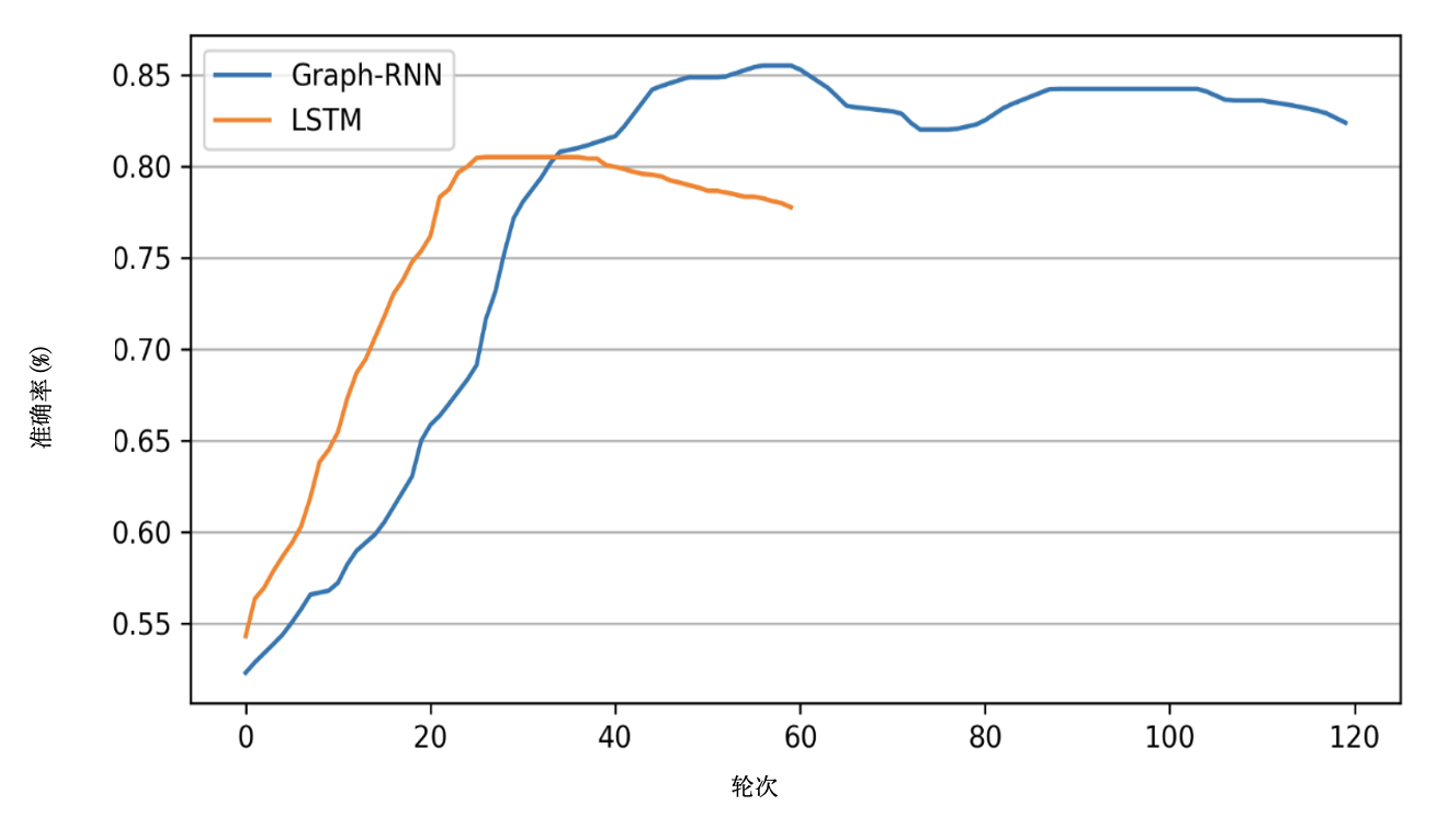
\includegraphics[width=1\linewidth]{accuracy_epoches.png}
    \caption{FG-RNN和LSTM准确率对比}
    \label{fig:FG-RNN和LSTM准确率对比}
  \end{figure}

图\ref{fig:FG-RNN和LSTM loss收敛对比}表示FG-RNN和LSTM两个算法loss收敛的对比,在达到稳定的准确率后,loss也会维持一个相对稳定的水平。
  \begin{figure}[H]
    \centering
    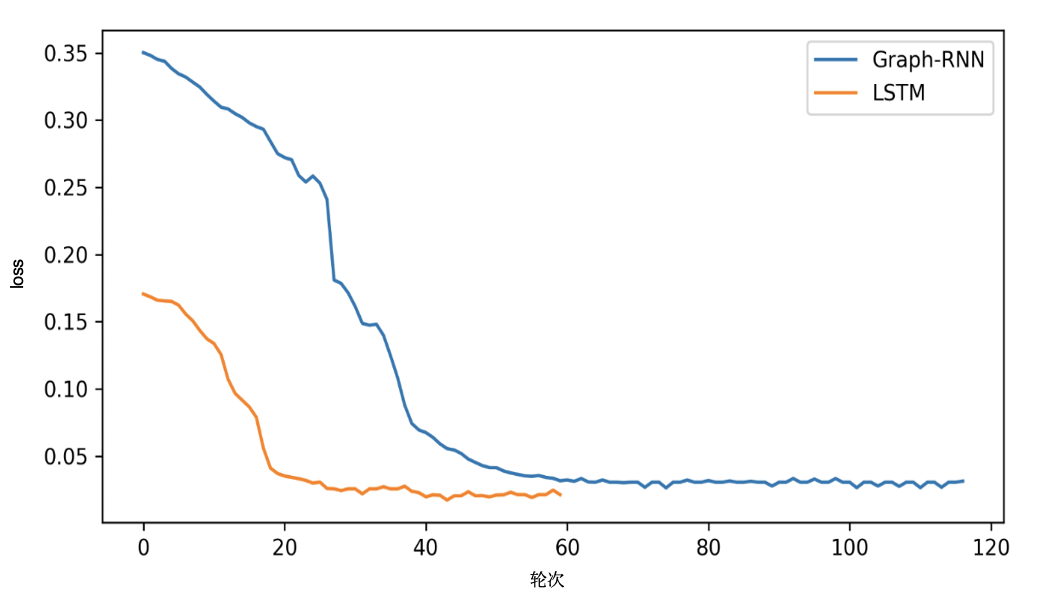
\includegraphics[width=1\linewidth]{loss_epoch.png}
    \caption{FG-RNN和LSTM loss收敛对比}
    \label{fig:FG-RNN和LSTM loss收敛对比}
  \end{figure}

\subsection{实验结果对比}
对于本文提出的模型和baseline模型,我们都进行了5次重复试验。从表\ref{不同数据集下实验评估结果FG}中可以看出,在UNSW-NB15和CICIDS2017数据集上,FG-RNN相比于基准模型没有明显提升,这可能是因为这两个数据集场景简单,各类算法的效果已经到达瓶颈。而在CAMPUS数据集上,FG-RNN明显好于LR、DT、RF这些基准模型,并且在基本的RNN类模型上提升巨大。该表格中使用的指标为准确率,为了全方位对比实验结果,我们从准确率、召回率、F1-score、运行时长等多方面进行了对比。结果如图3.10-3.13所示。本实验中除FG-RNN进行了超参数优化外,其余模型均使用默认参数,因此其他模型的效果可能仍有提升空间。
\begin{enumerate}
  \item 各类算法在开源数据集上的效果均要好于在CAMPUS数据集上的效果,这是因为CAMPUS数据集远比其余数据集更复杂。
  \item FG-RNN在准确率指标上比机器学习模型提升了约10.8\%,比深度学习模型提升了超过50\%,说明FG能够为RNN有效增加特征信息。
  \item 从召回率来看,相比于baseline模型,FG-RNN没有很好地提高召回率,说明该模型会发生很多“漏报”情况,后续我们更详细地分析了不同类别异常的召回率。
  \item F1-score兼顾了准确率和召回率的评估。由于召回率的影响,FG-RNN仅比机器学习模型提升了2\%的F1-score。后续工作可以考虑从提高召回率的角度优化模型。
  \item 由于数据集大小不同,对比同一算法在不同数据集上的运行时间没有意义。在相同数据集上,可以看出RNN类模型的训练时间要普遍比机器学习模型耗时更长,而FG-RNN又要消耗约两倍的时间,但是相比于准召和F1-score带来的提升,这些训练开销是可以接受的。
\end{enumerate}
\begin{table*}[h]
  \small
  \caption{不同数据集下实验评估结果(\%)}
  \label{不同数据集下实验评估结果FG}
  \centering
  \begin{tabular}{c|c|ccc|ccc|c}
  \toprule
  
    数据集 &  任务  &  
    LR &  DT & RF & RNN & LSTM & GRU & FG-RNN  \\
  \midrule
  
  UNSW-NB15 & 二分类 & 96.8 & 97.33 & 98.52 &  95.51 & 96.74 & 94.91 & 95.8 \\ 
  
  & 多分类 &94.73 & 97.96 & 96.82 & 93.98 & 92.11 & 94.30 & 94.24 \\
  
  \midrule
  CICIDS2017 & 二分类 & 98.26 & 97.11 & 95.54 & 90.18 & 88.04 & 91.49 & 92.45 \\
  & 多分类 & 97.01 & 97.37 & 94.41 & 88.31 & 91.16 & 90.18 & 90.67\\
  \midrule
  CAMPUS & 二分类 & 76.98 & 77.95 & 77.51 & 55.62 & 59.80 & 55.25 & 84.34 \\
  & 多分类 & 73.33 & 74.01 & 74.54 & 53.01 & 56.59 & 59.28 & 82.74\\
  
    \bottomrule
  
  \end{tabular}
  \end{table*}

  \begin{figure}[htbp]
    \centering
    \begin{minipage}[t]{0.48\textwidth}
    \centering
    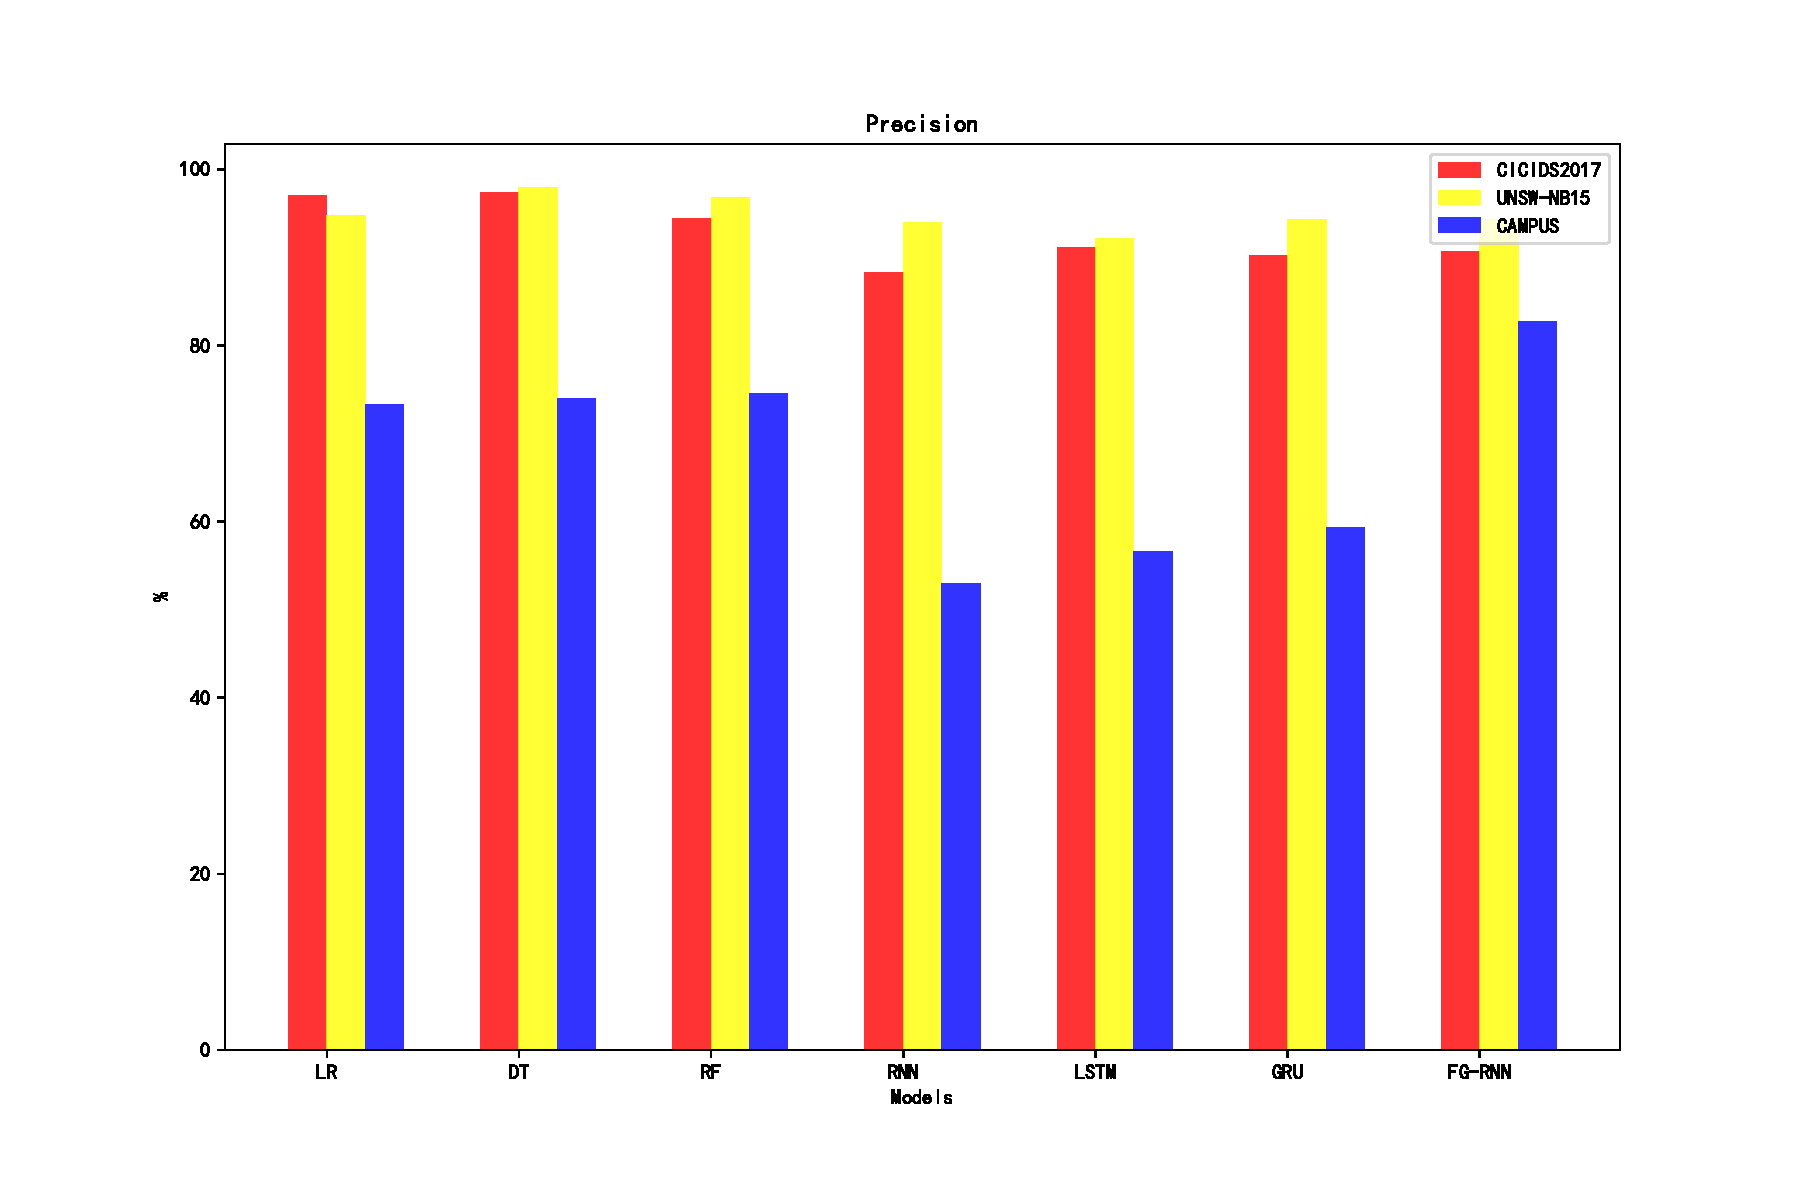
\includegraphics[width=1\linewidth]{实验结果对比-准确率.pdf}
    \caption{准确率对比}
    \end{minipage}
    \begin{minipage}[t]{0.48\textwidth}
    \centering
    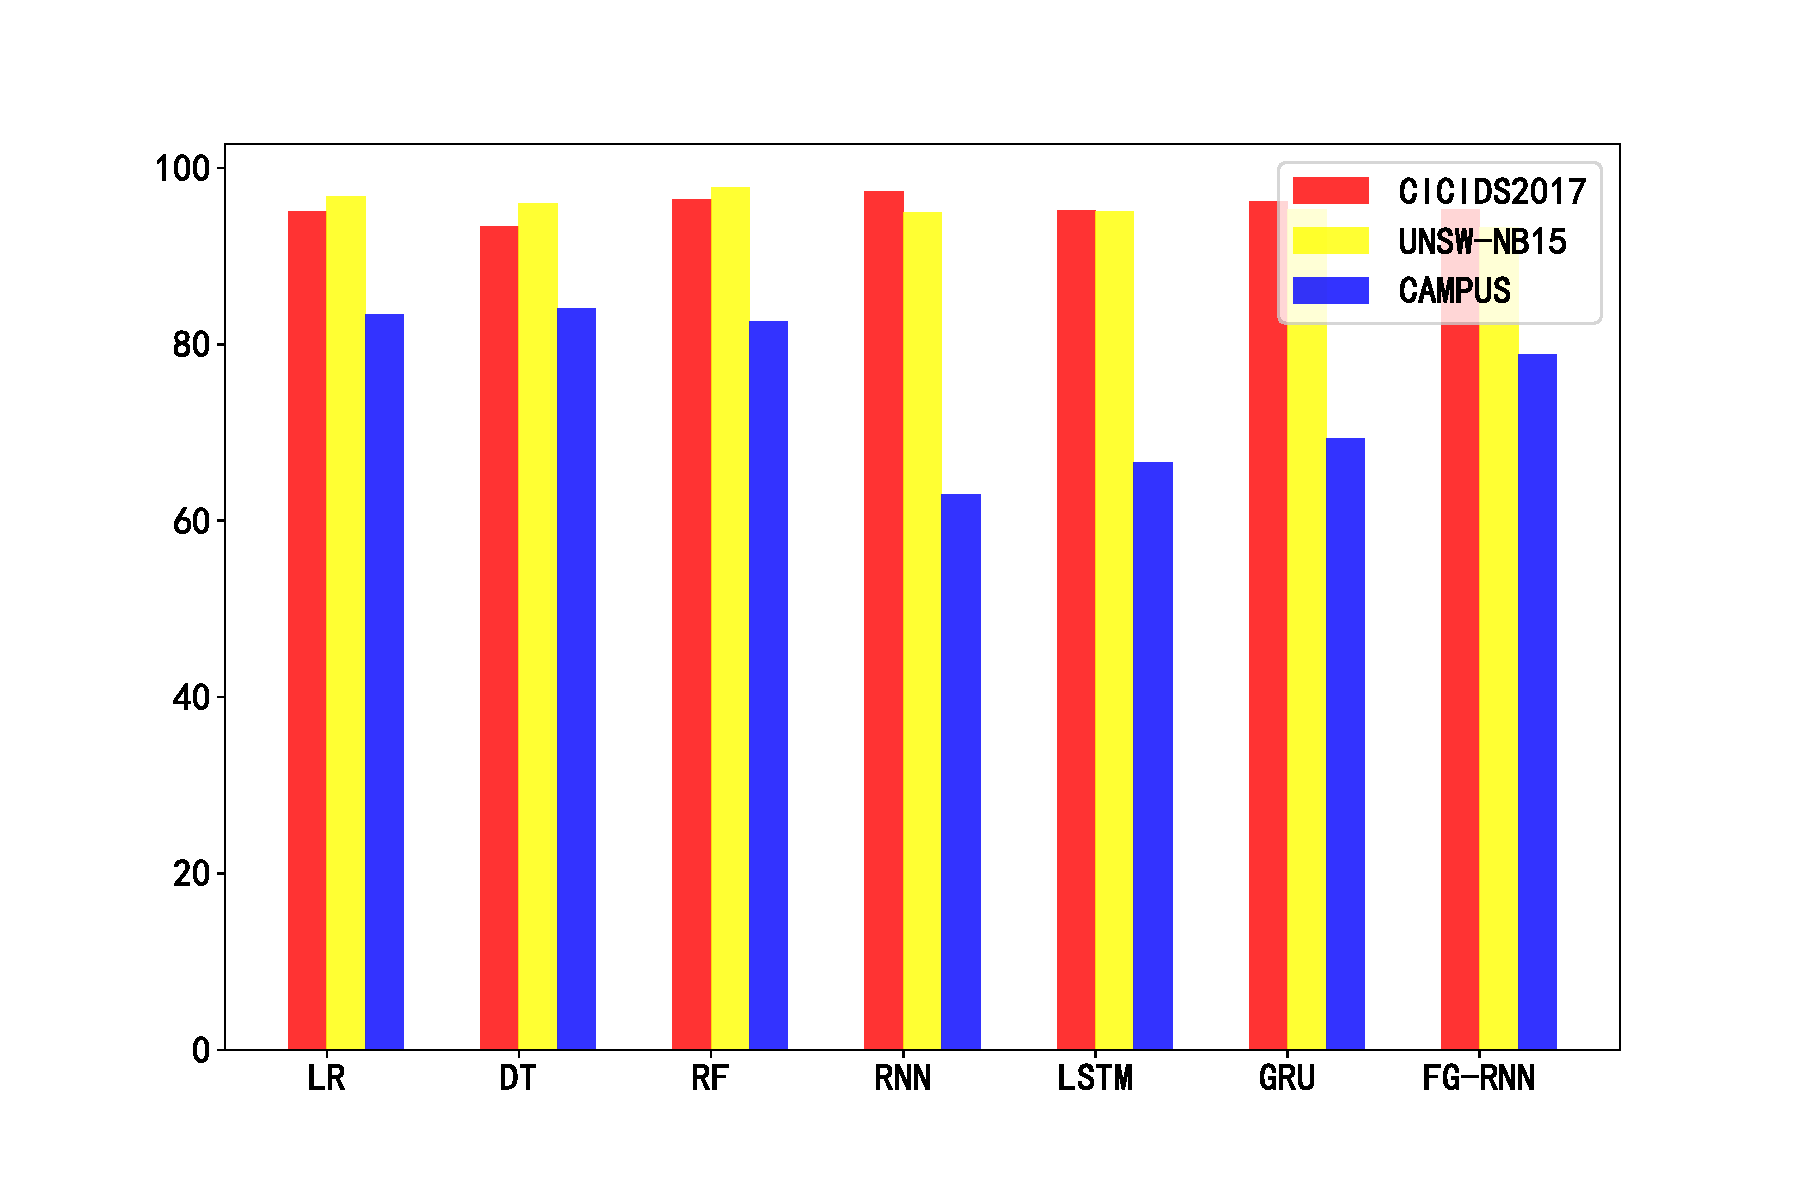
\includegraphics[width=1\linewidth]{实验结果对比-召回率.pdf}
    \caption{召回率对比}
    \end{minipage}
    \end{figure}

    \begin{figure}[htbp]
      \centering
      \begin{minipage}[t]{0.48\textwidth}
      \centering
      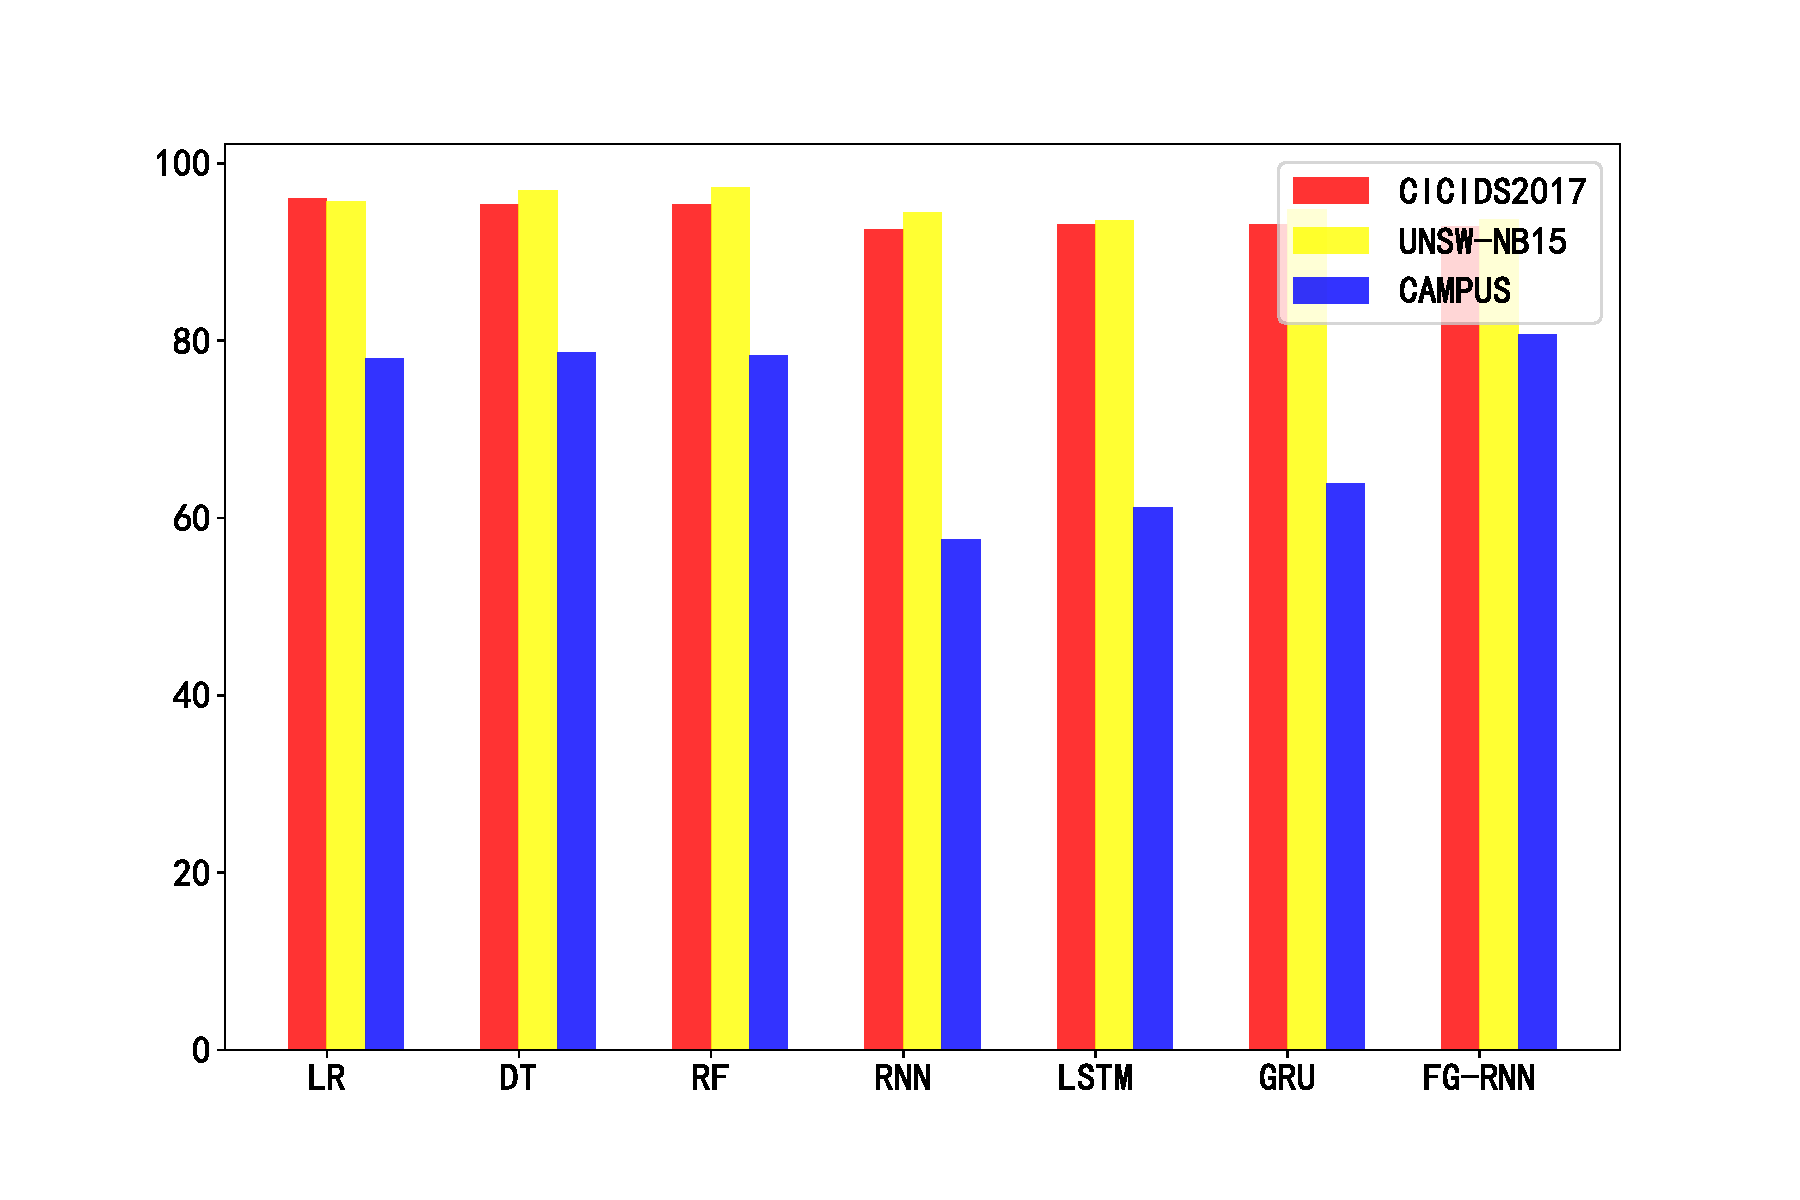
\includegraphics[width=1\linewidth]{实验结果对比-F1.pdf}
      \caption{F1 score对比}
      \end{minipage}
      \begin{minipage}[t]{0.48\textwidth}
      \centering
      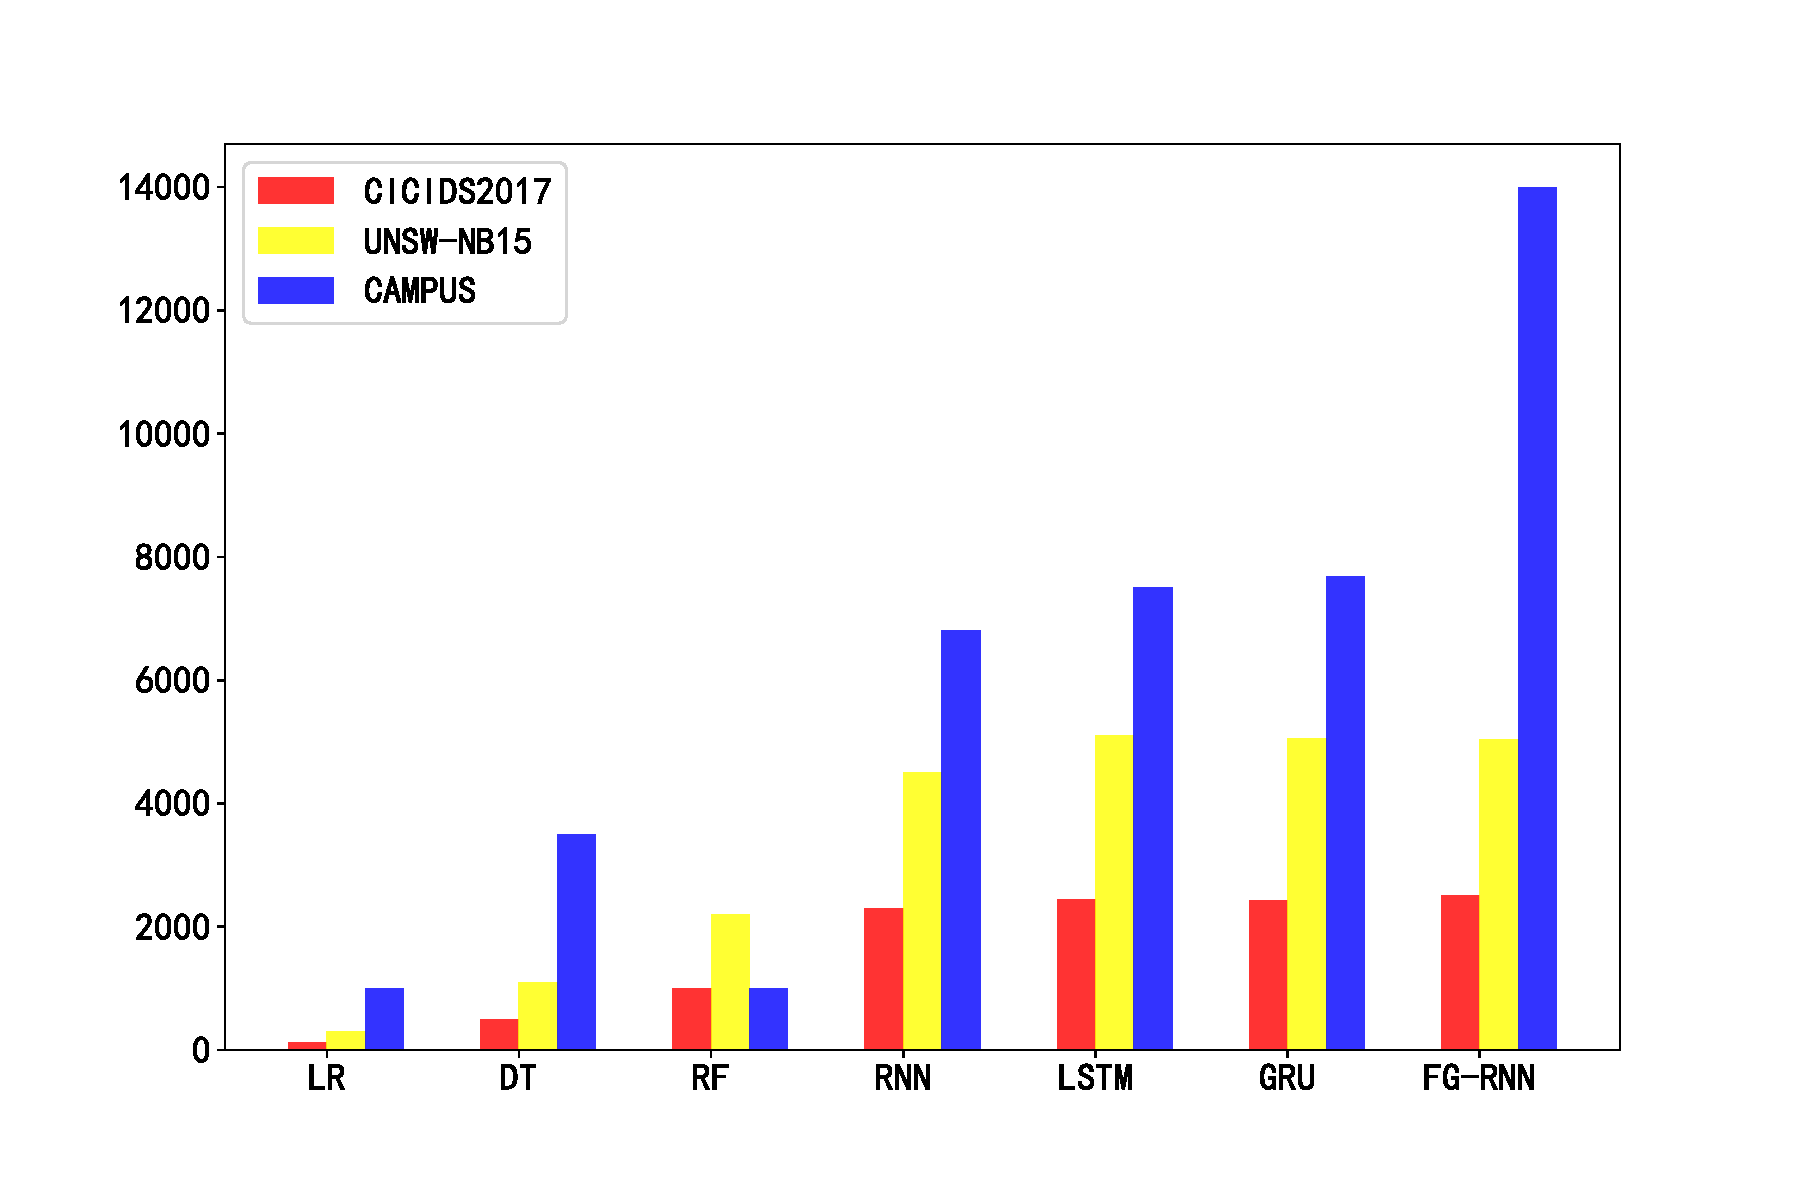
\includegraphics[width=1\linewidth]{实验结果对比-Time.pdf}
      \caption{运行时间对比}
      \end{minipage}
      \end{figure}
% \begin{figure}
%   \centering
%   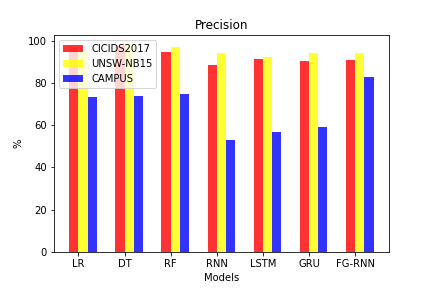
\includegraphics[width=0.6\linewidth]{实验结果对比-准确率.png}
%   \caption{实验结果对比-准确率}
%   \label{fig:实验结果对比-准确率}
% \end{figure}

% \begin{figure}
%   \centering
%   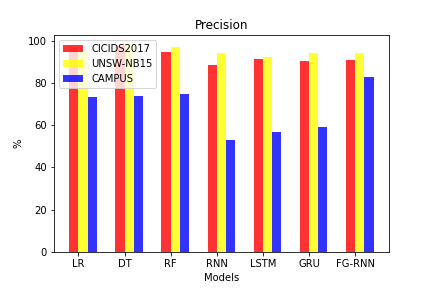
\includegraphics[width=0.6\linewidth]{实验结果对比-准确率.png}
%   \caption{实验结果对比-准确率}
%   \label{fig:实验结果对比-准确率}
% \end{figure}
% 僵尸网络:周期性强,规律性强;暴力猜解:时间间隔;拒绝服务; 流氓推广:大量下载行为,多个TCP流;
% 远控木马:大量上传行为;网络蠕虫:自动扩散
接下来,我们针对FG-RNN模型在CAMPUS数据集中的实验结果,具体分析了每种异常类型的准确率和召回率。将准确率定义为:
\begin{equation}
  P = \frac{\mbox{模型检测出的真正的异常量}}{\mbox{模型检测出的异常量}}
\end{equation}
召回率定义为:
\begin{equation}
  R = \frac{\mbox{模型检测出的真正异常量}}{\mbox{数据集中的全部异常量}}
\end{equation}
如图\ref{fig:不同异常类型的准召对比}所示,模型的准确率整体而言尚可,最低为远控木马类的76.3\%,最高为拒绝服务类的90.5\%,平均为82.7\%,这体现了模型检测结果误报率低的特点,检测结果具有较强的可信度。但是模型对于不同类型异常的召回率相差很大,远控木马仅为12\%,而暴力猜解为94.3\%,平均为78.8\%,以平均值作为分界线,高于平均值的类别有僵尸网络、暴力猜解、拒绝服务、流氓推广、端口扫描,低于平均值的类别有远控木马、网络蠕虫、代码执行,这些类别具有较强的伪装性,往往和正常流量的模式行为极为相似。从召回率可以看出,模型在检测某些特定异常时效果不佳,存在较严重的漏报,由于其余类别的召回率优于baseline模型,所以我们可以将这些特定异常类别的检测结果仅作为参考。这部分缺陷也是我们未来工作中进行优化的方向。

% 因为暴力猜解的流量特征比较明显,可以很容易学习到特征,远控木马的特点是,僵尸网络:周期性强,规律性强;暴力猜解:时间间隔;拒绝服务; 流氓推广:大量下载行为,多个TCP流;
% 远控木马:大量上传行为;网络蠕虫:自动扩散

\begin{figure}
  \centering
  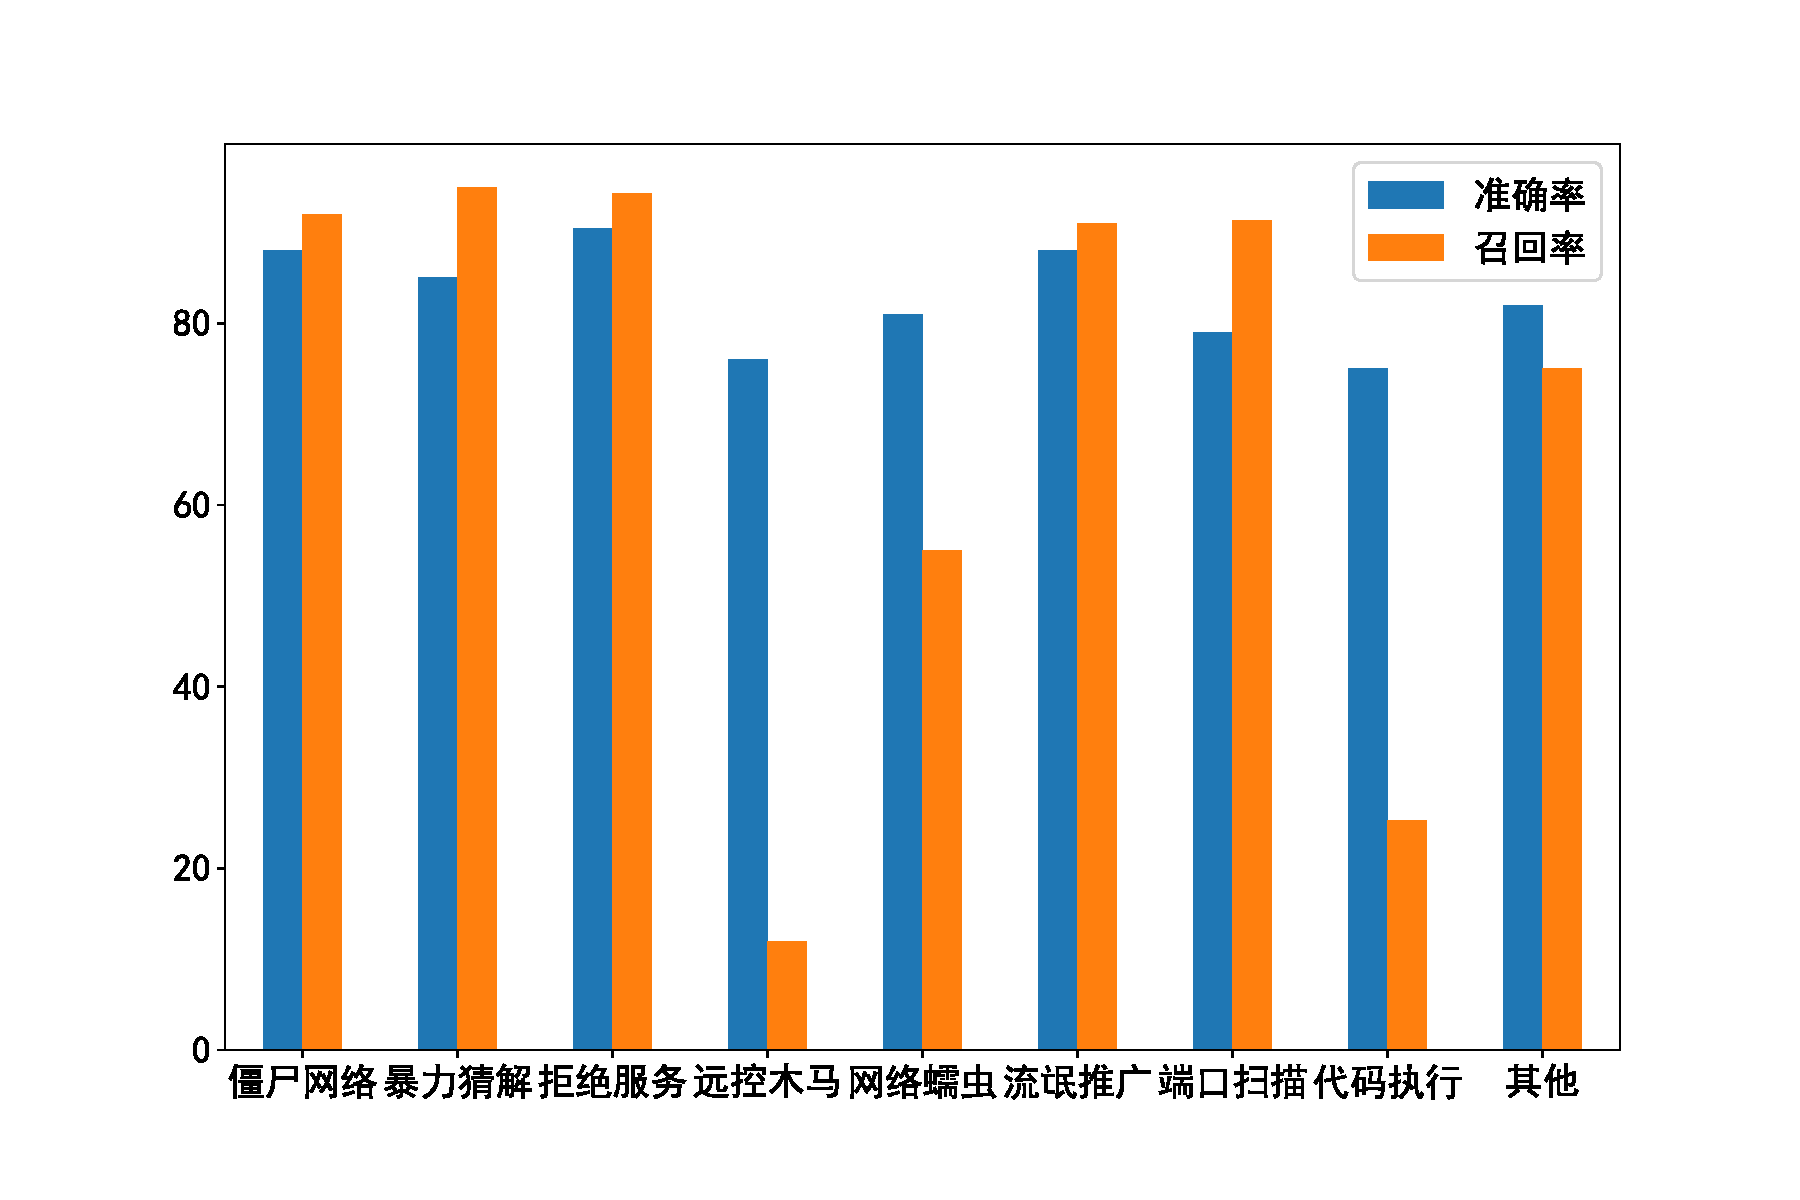
\includegraphics[width=1\linewidth]{不同异常类型的准召对比.pdf}
  \caption{不同异常类型的准召对比}
  \label{fig:不同异常类型的准召对比}
\end{figure}

\section{本章小结}
为应对校园网流量环境的复杂情况,本章首先针对不同算法进行了特征分析,找出RNN在CAMPUS数据集中表现不佳的原因,然后设计了基于特征关系图的RNN算法,最后在多个数据集上进行了实验评估。
% 根据第3章的实验结果,LSTM和GRU在CAMPUS数据集下准确率仅为65.4\%和67.8\%,而加入固定的特征关系图后,LSTM准确率即可达到81.2\%,将特征关系图与RNN同时训练,动态更新特征关系矩阵的参数,则FG-RNN算法的准确率可达到85.3\%。


% \subsection{基于真实数据的检测结果}
% 交叉熵损失函数经常用于分类问题中,特别是在神经网络做分类问题时,也经常使用交叉熵作为损失函数,此外,由于交叉熵涉及到计算每个类别的概率,所以交叉熵几乎每次都和sigmoid(或softmax)函数一起出现。

% 我们用神经网络最后一层输出的情况,来观察整个模型预测、获得损失和学习的流程:

% 神经网络最后一层得到每个类别的得分scores;
% 该得分经过sigmoid(或softmax)函数获得概率输出;
% 模型预测的类别概率输出与真实类别的one hot形式进行交叉熵损失函数的计算。
% \begin{figure}
%   \centering
%   
\includegraphics[width=0.6\linewidth]{example-image-a.pdf}
%   \caption{Example figure in appendix}
%   \label{fig:appendix-survey-figure}
% \end{figure}




